\chapter{\label{ch:ch02}ГЛАВА 2: Знакомство с интерфейсом <<Godot>>}

\section{\label{sec:ch02/sec01}Установка <<Godot>>}

\subsection{\label{subsec:ch02/sec01/sub01}Переход на сайт}
Установить наш движок мы можем несколькими методами:
\begin{itemize}
    \item Через Steam
    \item Через официальный сайт
\end{itemize}


\begin{figure}[h]
    \centering
    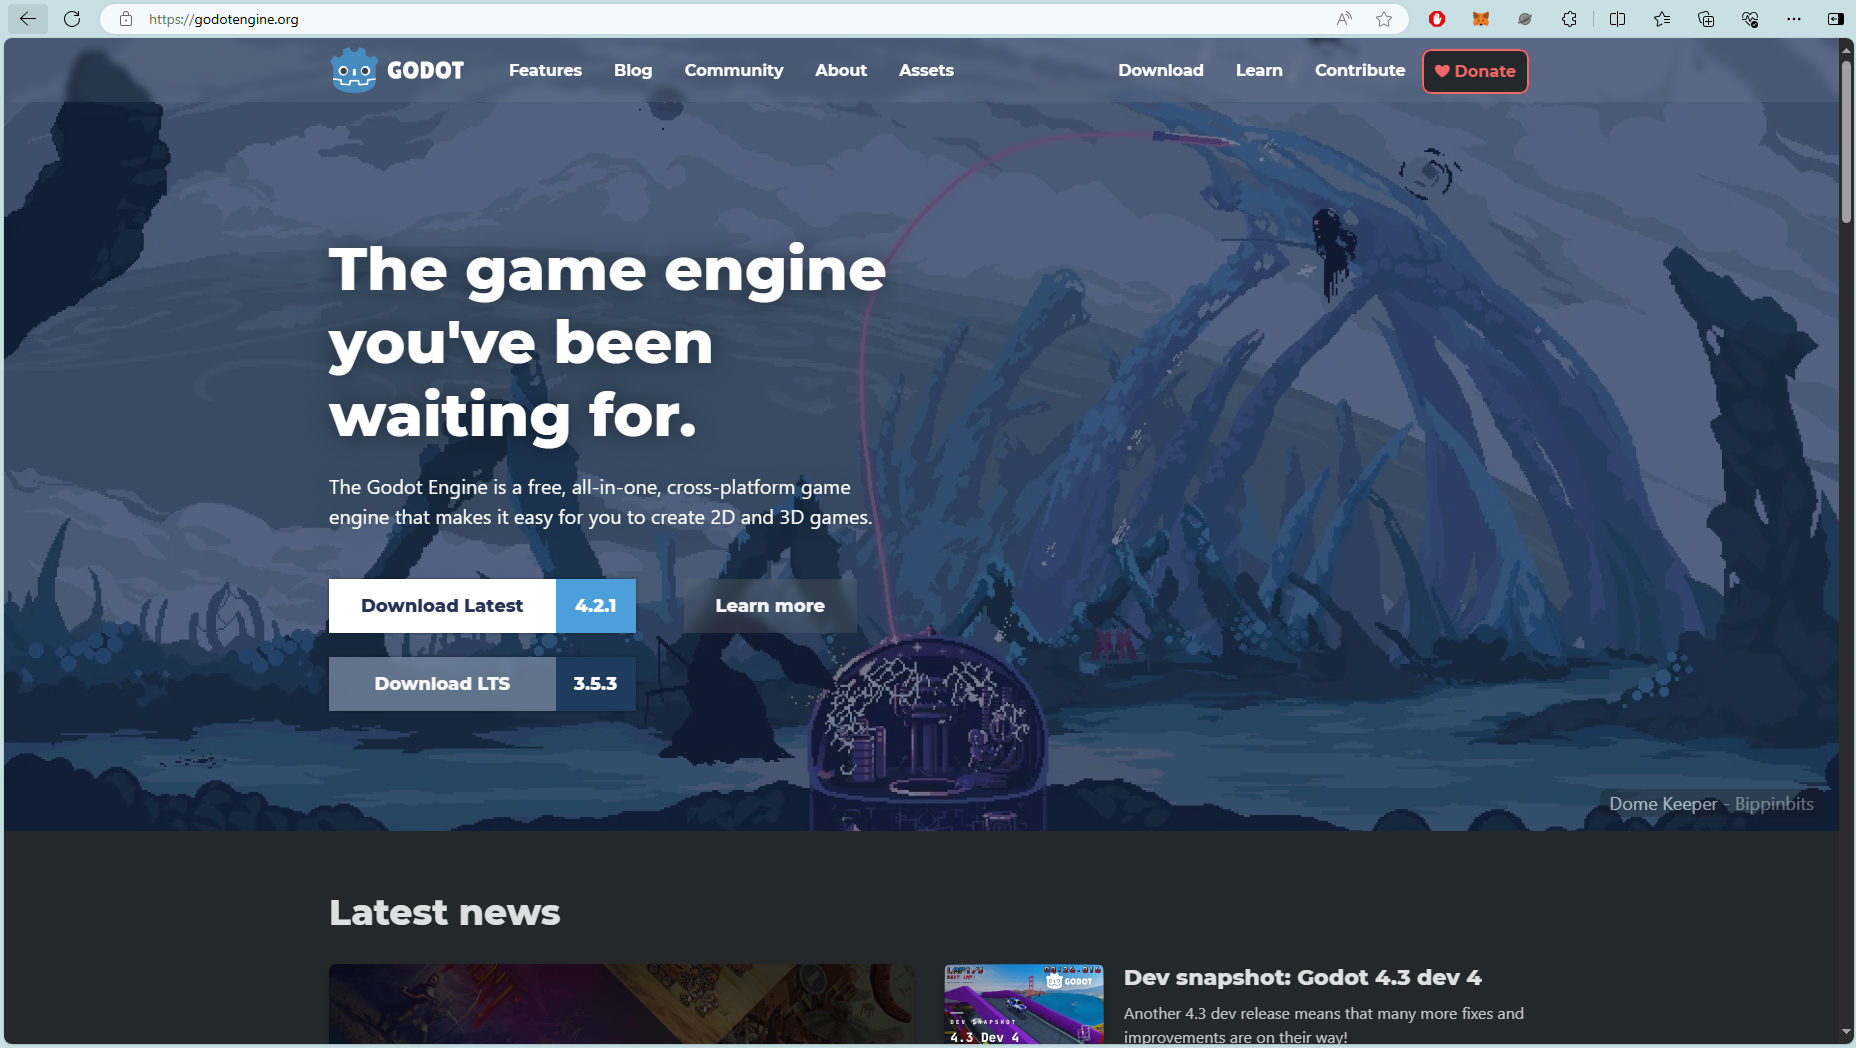
\includegraphics[width=1\textwidth]{images/godotsait.png}
\caption{\centering\label{fig:example03}Официальный сайт <<Godot>>.}
\end{figure}


\begin{figure}[h]
    \centering
    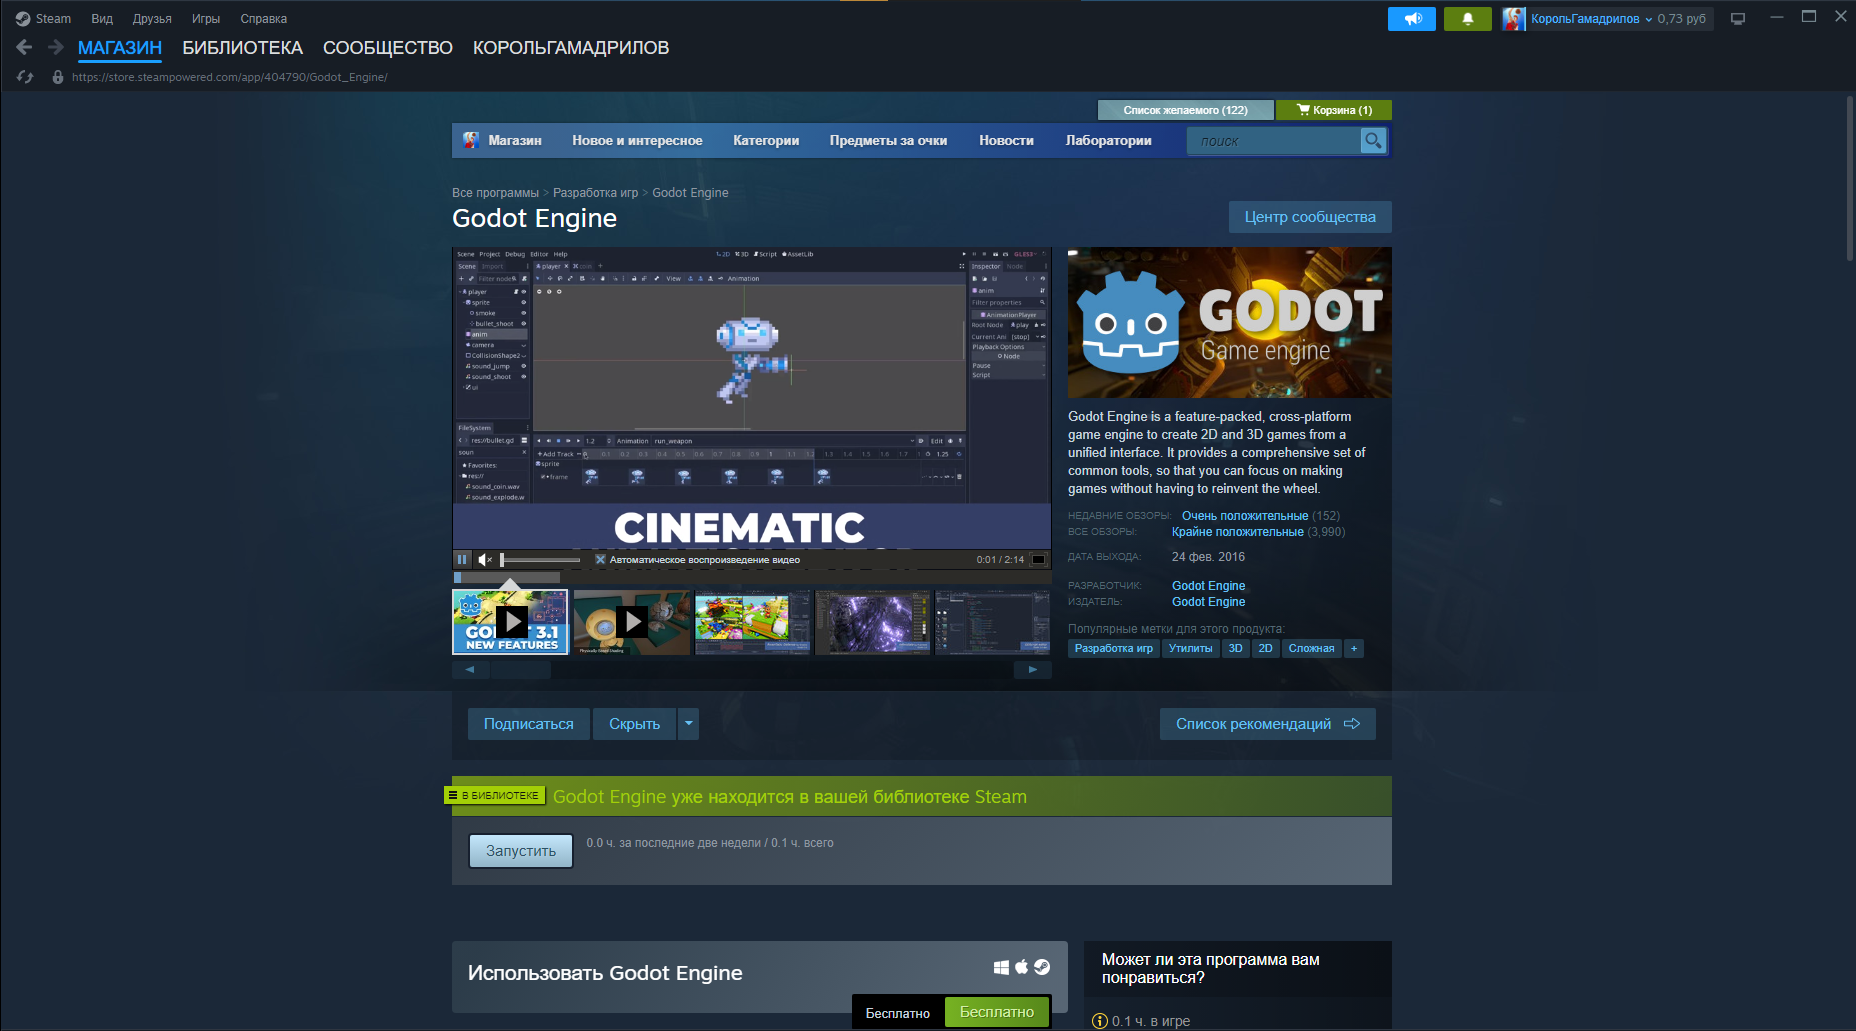
\includegraphics[width=1\textwidth]{images/godotSteam.png}
\caption{\centering\label{fig:example04}Официальная страница <<Godot>> в Steam.}
\end{figure}


\subsection{\label{subsec:ch02/sec02/sub01}Создание проекта}
Как только мы установили <<Godot>> на наш пк, мы открываем его и вот что нас встречает:
\section{\label{sec:ch02/sec02}Интерфейс программы}

\begin{figure}[h]
    \centering
    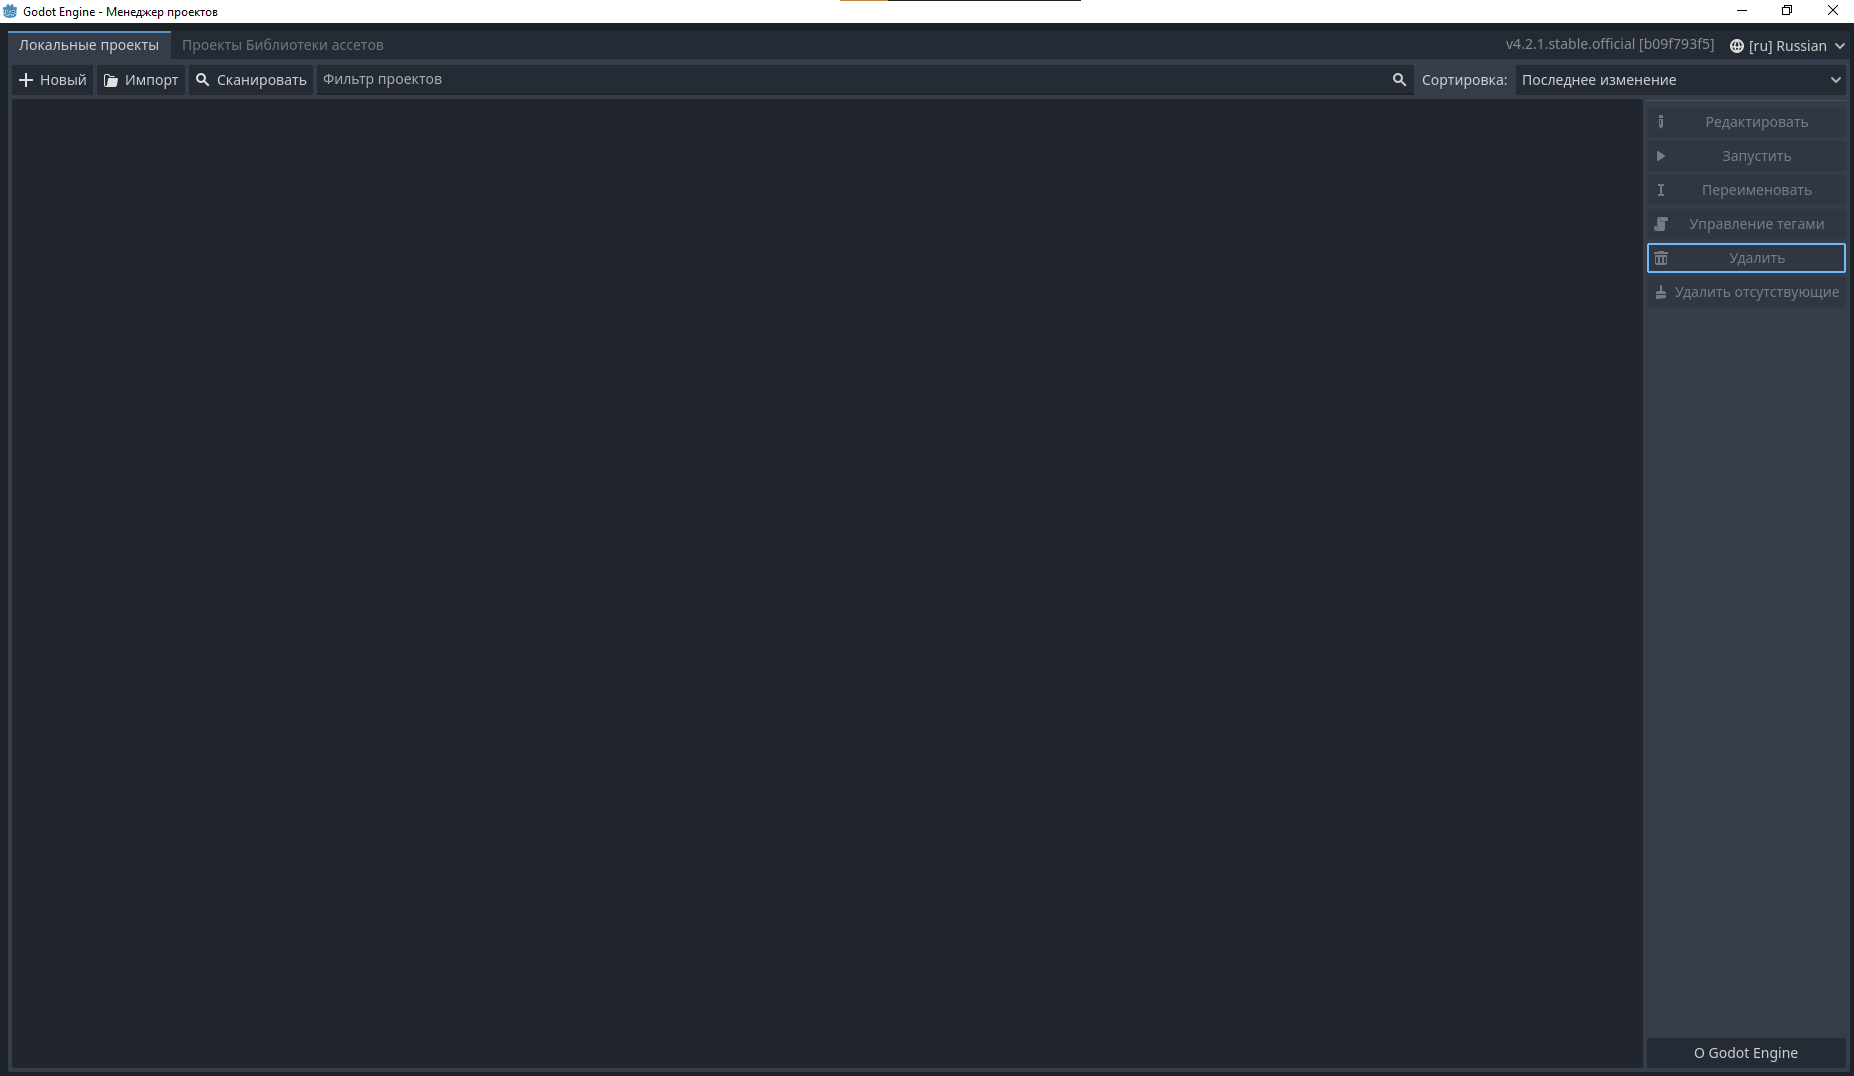
\includegraphics[width=1\textwidth]{images/Менеджер проектов.png}
\caption{\centering\label{fig:example05}Менеджер проектов.}
\end{figure}
